% !TEX TS-program = XeLaTeX
% Commands for running this example:
% 	 xelatex Vahid-Proposal
% 	 xelatex Vahid-Proposal
% End of Commands

%%%  نمونه یک پروپوزال کارشناسی ارشد

% توجه داشته باشید برای دیدن خروجی کامل شامل نمایه و فهرست مطالب در ویرایشگر Texmaker، ابتدا دو بار 
% کلید F1 و بعد کلید F12 و دوباره کلید F1 و در آخر کلید F7 را فشار دهید.
%توضیحات مربوط به هر بسته یا دستور را می‌توانید در خط بالای آن ببینید.

\documentclass[12pt,a4paper,oneside]{book}
\usepackage[top=40mm, bottom=40mm, left=25mm, right=35mm]{geometry}
\usepackage{fancyhdr}
%در ورژن جدید زی‌پرشین برای تایپ متن‌های ریاضی، این سه بسته، حتماً باید فراخوانی شود
\usepackage{amsthm,amssymb}
\usepackage[table]{xcolor}% http://ctan.org/pkg/xcolor
\usepackage{float}
%دستوری برای وارد کردن واژه‌نامه انگلیسی به فارسی
\newcommand\persiangloss[2]{#1\dotfill\lr{#2}\\}
%بسته‌ای برای تنطیم حاشیه‌های بالا، پایین، چپ و راست صفحه
%\usepackage[top=50mm, bottom=50mm, left=50mm, right=50mm]{geometry}
%بسته‌ای برای نمایش تصاویر قرار داده شده در متن
\usepackage{graphicx}
\usepackage{standalone}
\usepackage{tikz}
\usetikzlibrary{shapes,arrows}
\usepackage[ruled]{algorithm}
\usepackage{algorithmic}
\usepackage{pgfplots}
\pgfplotsset{compat=newest}
\usepackage{standalone}
\usepackage{caption}
\usepackage{subcaption}
% بسته‌ و دستوراتی برای ایجاد لینک‌های رنگی با امکان جهش
\usepackage[pagebackref=false,colorlinks,linkcolor=blue,citecolor=blue]{hyperref}
% چنانچه قصد پرینت گرفتن نوشته خود را دارید، خط بالا را غیرفعال و  از دستور زیر استفاده کنید چون در صورت استفاده از دستور زیر‌‌، 
% لینک‌ها به رنگ سیاه ظاهر خواهند شد و برای پرینت گرفتن، مناسب‌تر خواهد بود
%\usepackage[pagebackref=false]{hyperref}
%بسته‌ای برای ظاهر شدن «مراجع» و «نمایه» در فهرست مطالب
\usepackage{tocbibind}
\usepackage{notoccite}
%دستورات زیر جهت هماهنگ شده با قالب دانشگاه علم و صنعت اضافه شده است.
\usepackage[fleqn]{amsmath}
\usepackage{titlesec}
%%%%%%%%%%%%%%
%فراخوانی بسته زی‌پرشین و دستورات مربوط به نوع فونت‌ها
\usepackage{fontspec}
\usepackage{xepersian}
\settextfont[Path = ./fonts/,Scale=1]{XB Niloofar}
% از revision 118 زی‌پرشین به بعد، وارد کردن دستور زیر لازم نیست. توجه داشته باشید که در صورت  غیرفعال کردن این دستور،
% از فونت پیش‌فرض لاتک برای کلمات انگلیسی استفاده خواهد شد.
%\setlatintextfont[ExternalLocation,BoldFont={lmroman10-bold},BoldItalicFont={lmroman10-bolditalic},ItalicFont={lmroman10-italic}]{lmroman10-regular}
% چنانچه می‌خواهید که اعداد در فرمول‌ها، فارسی باشد، دستور زیر را فعال کنید
%\setdigitfont{XB Zar}
%%%%%%%%%%%%%%%%%%%%%%%%%%%%%%%%%%%%%%%%%%%%%%%%%%%
% تعریف قلم‌های فارسی و انگلیسی برای استفاده در بعضی از قسمت‌های متن
\defpersianfont\titr[Path = ./fonts/,Scale=1]{XB Titre}
\defpersianfont\nastaliq[Path = ./fonts/,Scale=1.5]{XB Niloofar}
%\defpersianfont\traffic[Scale=1]{B Traffic}
%\defpersianfont\yekan[Scale=1]{B Yekan}
%اگر فونت‌های بالا را ندارید، دو خط بالا را غیر فعال و دو خط زیر را فعال کنید
\defpersianfont\traffic[Path = ./fonts/,Scale=1]{XB Roya}
\defpersianfont\yekan[Path = ./fonts/,Scale=1]{XB Kayhan}
%%%%%%%%%%%%%%%%
%%%%%%%%%%%%%%%%

\newcommand{\norm}[1]{\left\lVert#1\right\rVert}


\theoremstyle{definition}
\newtheorem{definition}{تعریف}
\newtheorem{theorem}{قضیه}
\newtheorem{lemma}{لم}
\newtheorem{proposition}{گزاره}
\newtheorem{corollary}{نتیجه}
\newtheorem{remark}{ملاحظه}
\theoremstyle{definition}
\newtheorem{example}{مثال}
%%%%%%%%%%%%%%%%%%


\pagestyle{fancy}
\fancyhf{}

\fancyhead[LE,LO]{\nouppercase{\leftmark}}
\fancyfoot[C]{\thepage}

\renewcommand\headrulewidth{1.5pt}
\makeatletter
\def\headrule{{\if@fancyplain\let\headrulewidth\plainheadrulewidth\fi
\hrule\@height\headrulewidth\@width\headwidth
\vskip 2pt% 2pt between lines
\hrule\@height.5pt\@width\headwidth% lower line with .5pt line width
\vskip-\headrulewidth
\vskip-1.5pt}}
\makeatother

%%%%%%%%%%%%%%%%%%
\SepMark{-}
%%%%%%%%%
 \titleformat{\chapter}[display]
{\vspace{-3cm}\vfill\filcenter}
{{%
   \vspace{-3cm}\filcenter\fontsize{48pt}{48pt}\selectfont{\chaptername}
   \fontsize{48pt}{48pt}\selectfont\thechapter%
 }%
}
{50pt}
{\fontsize{30pt}{30pt}\selectfont%
}[\vfill\clearpage]
\titlespacing*{\chapter}{0pt}{0pt}{0pt}
%%%%%%%%%%%%%%%%
%%%%%%%%%%%%%% HB %%%%%%%%%%%%%%%%
\usepackage{bm}
\usepackage[font=scriptsize,labelfont=bf]{caption}
\usepackage{perpage}
 \MakePerPage{footnote}
%%%%%%%%%%%%%% HB %%%%%%%%%%%%%%%%
\def\C{ \mathbb{C}}
\def\R{\mathbb{R}}
\def\Z{ \mathbb{Z}}
\def\N{ \mathbb{N}}

%%%%%%%%%%%%%%%%

\begin{document}

% دستوری جهت ظاهر نشدن شماره صفحه و سربرگ، در صورت وجود (فقط در صفحه جاری)
\thispagestyle{empty}
\vspace*{-28mm}
% نحوه درج کردن لوگوی دانشگاه
\centerline{
\includegraphics[scale=0.1]{./Images/general/logo.png}}
\begin{center}
%دستوری برای کم کردن فاصله بین لوگو و خط پایین آن
\vspace{-1mm}
\textbf{دانشکده فنی و مهندسی}
%دستوری برای تعیین فاصله بین دو خط
\\[3cm]
\begin{Huge}
\textbf{
بررسی و کاهش کوپلینگ متقابل در آنتن های میکرواستریپ
}
\end{Huge}
\\[1.5cm]
\Large
گزارش پایانی پروژه‌ی کارشناسی
\\[0.25cm]
در رشته‌ی مهندسی برق گرایش مخابرات
\\[3cm]
دانشجو:
\\[0.25cm]
\textbf{
محمد حسن بهشتی    
\\[1cm]
استاد راهنما:
\\[0.25cm]
دکتر حمیدرضا حسنی
\\[1cm]
شهریور ماه ۱۴۰۴
}
\end{center}
\newpage
\thispagestyle{empty}
\centerline{\includegraphics[scale=0.75]{./Images/general/besmallah.jpg}}

\newpage
\thispagestyle{empty}
\centerline{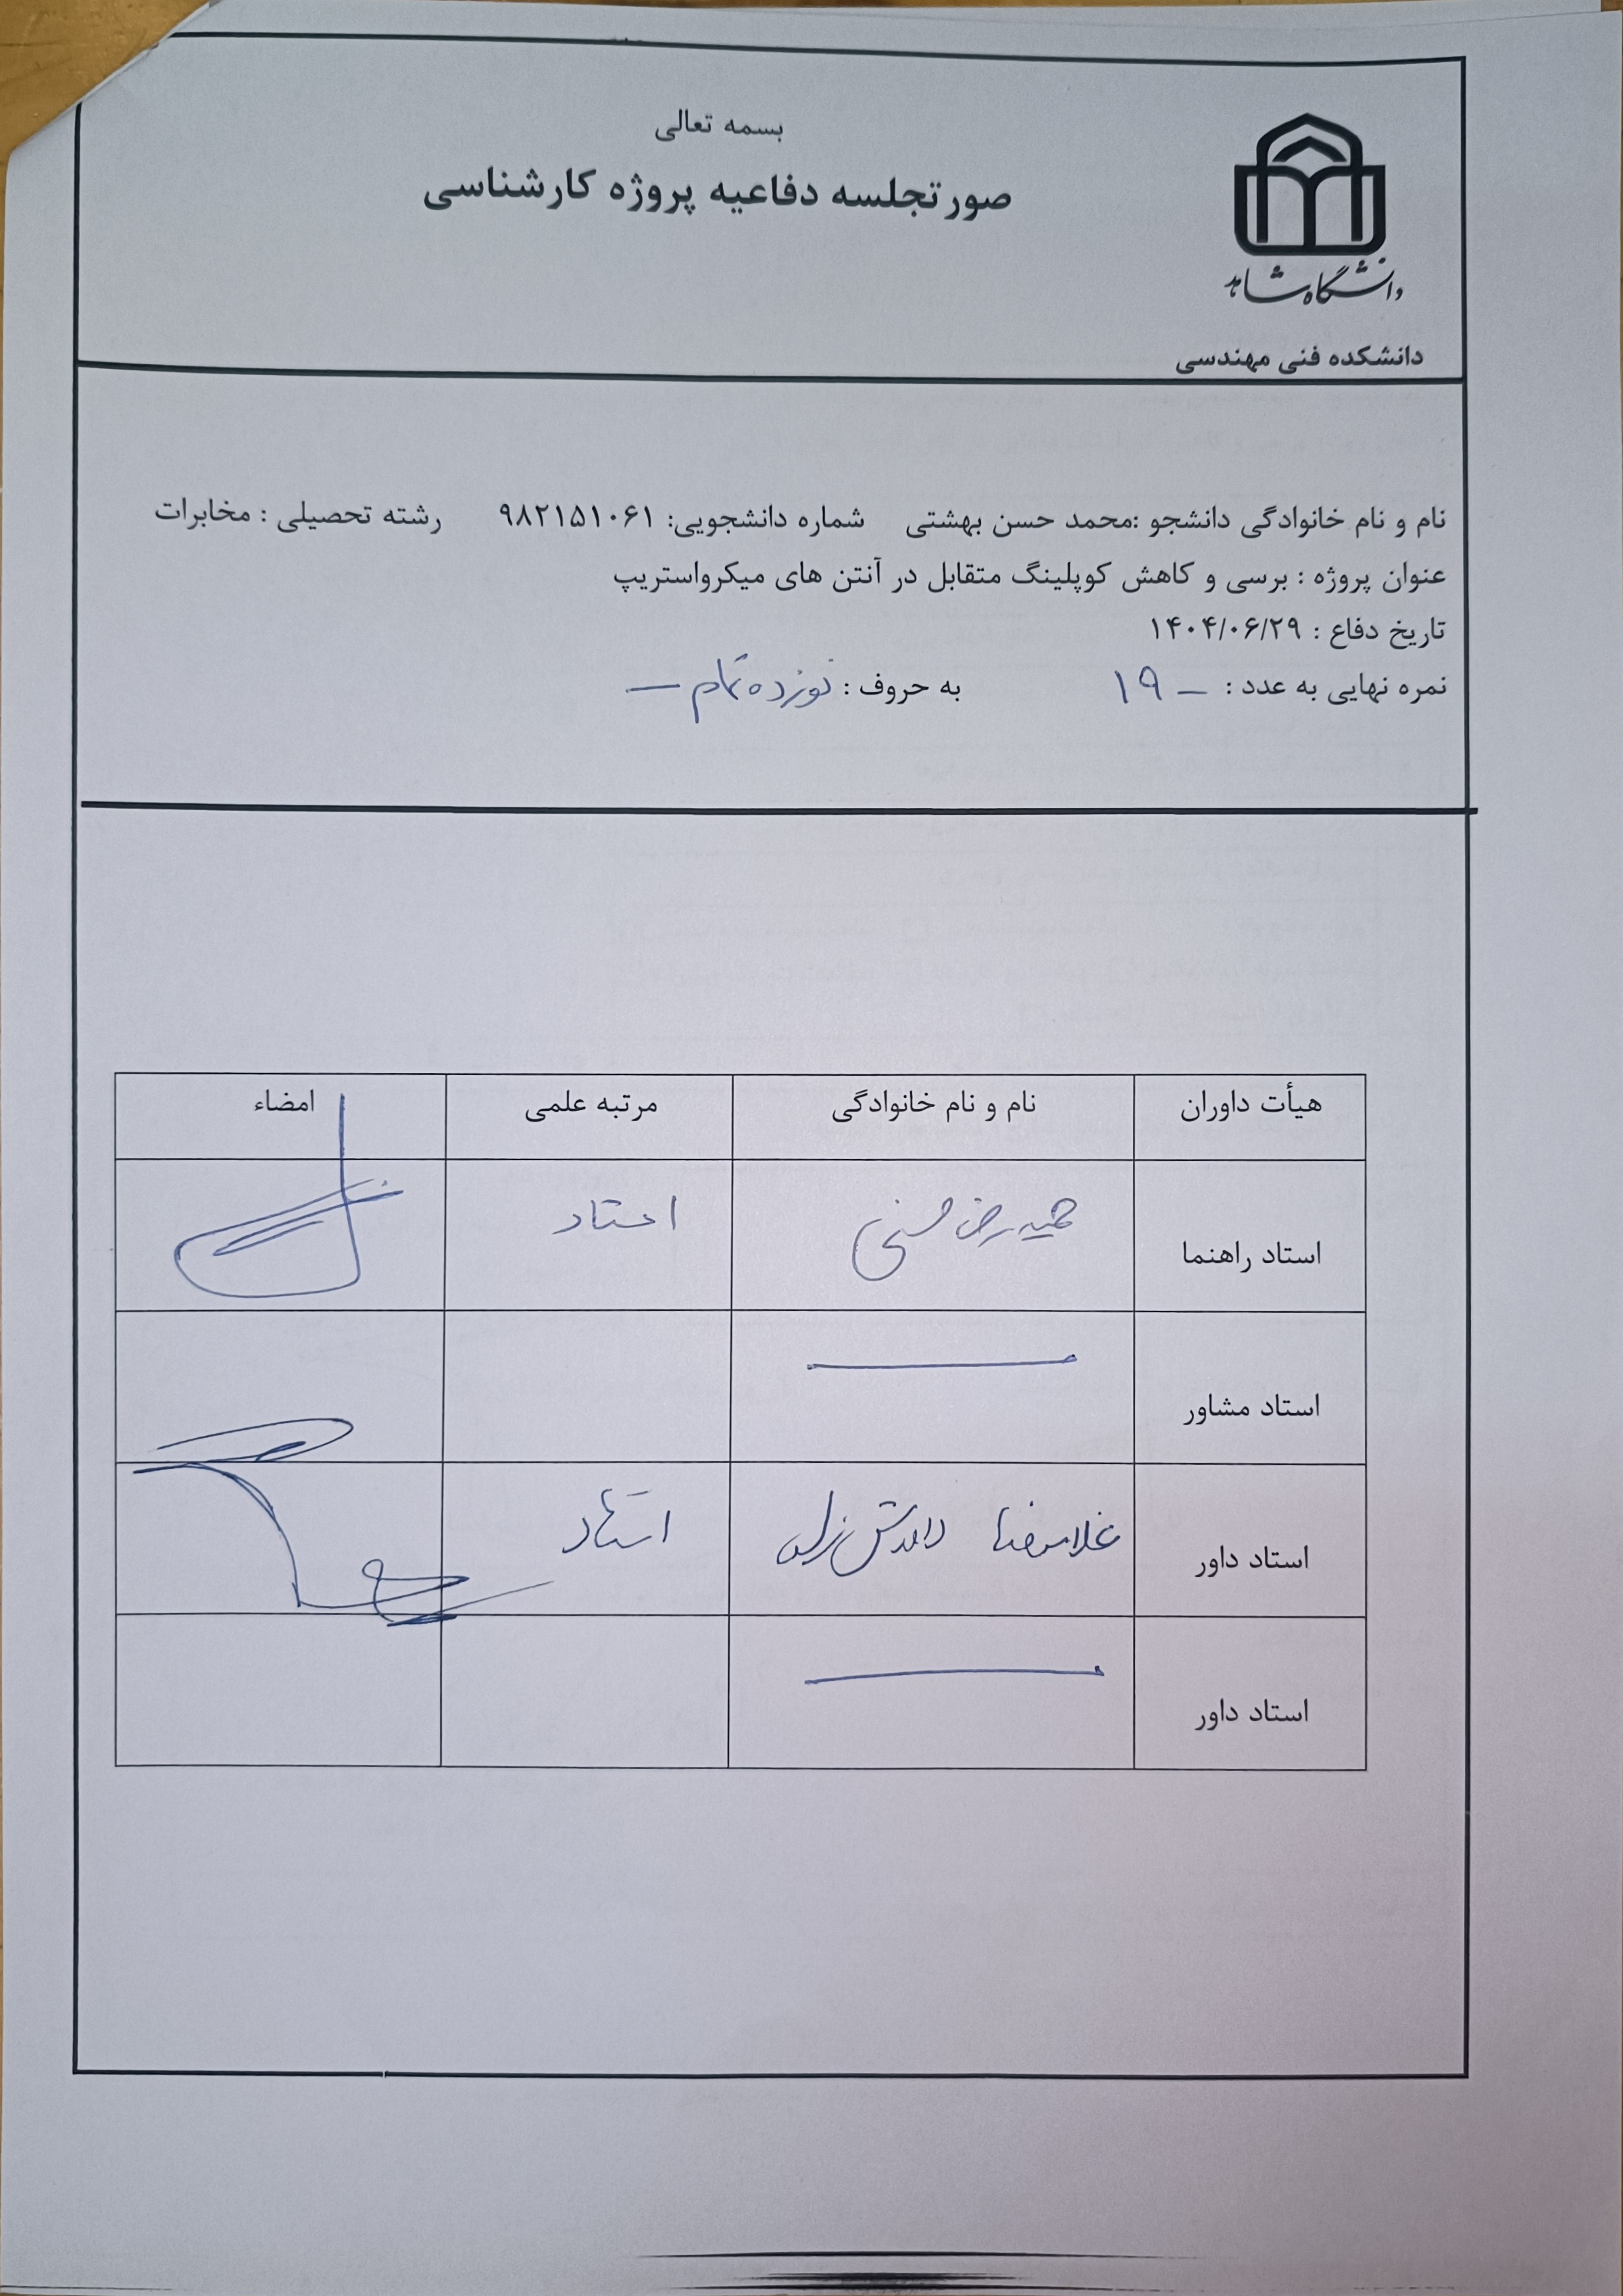
\includegraphics[scale=0.2]{./Images/general/soorat.jpg}}
\pagenumbering{harfi}
%دستوری برای ظاهر شدن فهرست مطالب
\tableofcontents
\newpage
\listoffigures

\baselineskip=1cm
\newpage 
\chapter*{چکیده}
\thispagestyle{empty}
\section*{چکیده}

آنتن‌های میکرواستریپ به دلیل سادگی ساخت و ابعاد کوچک کاربرد وسیعی در سامانه‌های مخابراتی دارند. با این حال، استفاده از آن‌ها در قالب آرایه موجب تزویج متقابل میان عناصر می‌شود که پیامدهایی همچون افت بهره و اعوجاج الگوی تشعشعی را به همراه دارد. در این پژوهش، برای بررسی و کاهش این اثر پس از معرفی آنتن مایکرواستریپ و آنتن آرایه ای، ابتدا مدل کلاسیک 
\lr{Carver \& Jedlicka}\cite{carver1981microstrip}
 شامل دو پچ مستطیلی در فواصل مختلف بازتولید گردید. سپس با پایه ی مقاله ی کارور در فاصله‌ی یک‌چهارم طول‌موج در فرکانس
\lr{1.41 GHz}
   و با الهام از مقاله
\cite{hajilou2012mutual}،
     یک ساختار
\lr{DGS}
       طراحی و اعمال شد. در ادامه، یک متاسرفیس با فاصله از صفحه ی آنتن، میان دو آنتن قرار گرفت تا با ایجاد باند توقف امواج سطحی، کوپلینگ بیشتر کاهش یابد. نتایج شبیه‌سازی در 
       \lr{HFSS}
        نشان داد که ترکیب
\lr{DGS}\LTRfootnote{Defected ground structure}
          و متاسرفیس موجب کاهش تا حدود 32 دسی‌بل در 
$\vert\bm{S}\vert_{21}$
در حالی که 
$\vert\bm{S}\vert_{11}$
 و الگوی اصلی تشعشعی تقریباً ثابت ماندند. این نتایج نشان‌دهنده‌ی کارآمدی فراساختارها در بهبود عملکرد آرایه‌های میکرواستریپ است.
 
 
\textbf{
کلمات کلیدی:
}
آنتن میکرواستریپ، کوپلینگ متقابل، کاهش کوپلینگ، آنتن‌های پچ، آنتن‌های میکروپچ


\pagenumbering{arabic}
\newpage 
\chapter{ آنتن های مایکرواستریپ}
\label{ch:1}

\section{مقدمه}
آنتن‌های مایکرواستریپ به دلیل برخورداری از مزایای متعددی همچون عملکرد مناسب، وزن سبک، قابلیت نصب آسان و هزینه تولید پایین، جایگاه ویژه‌ای در صنایع پیشرفته از جمله هوافضا، ماهواره‌ها و سیستم‌های ارتباطی پیدا کرده‌اند. ساختار چاپی این آنتن‌ها امکان یکپارچه‌سازی آسان با مدارات مایکروویو را فراهم می‌کند. پارامترهای اساسی عملکردی این آنتن‌ها از جمله فرکانس تشدید، الگوی تابشی و امپدانس ورودی عمدتاً توسط ابعاد هندسی پچ، ویژگی‌های زیرلایه و روش تغذیه تعیین می‌شوند. این فصل به ارائه مبانی تئوری، بررسی ویژگی‌ها، مزایا و محدودیت‌های این آنتن‌ها و همچنین تحلیل روش‌های مختلف تغذیه می‌پردازد.
\section{ویژگی های آنتن مایکرواستریپ}


در آنتن‌های مایکرواستریپ، ضخامت پَچ
\LTRfootnote{Patch}
 بسیار نازک است (
$ h \ll \lambda_{0}$
، که 
$ \lambda_{0} $
 طول موج در خلأ است) و ضخامت زیرلایه
\LTRfootnote{Substrate}
  کسری از طول موج است(رابطه 
 \eqref{eq:eq1}
 ). پَچ در بالای لایه زمین قرار گرفته و این دو توسط یک زیرلایه دی‌الکتریک از هم جدا شده‌اند. 
\begin{align}
	\label{eq:eq1}
	0.003\lambda_{0} < h < 0.05\lambda_{0}
\end{align}

در پَچ مستطیلی، اندازه ضلع
\lr{($L$)}
  در محدوده
$ \lambda_{2}/2 < L < \lambda_{2}/3$
    قرار دارد (که
$ \lambda_{2} $
      طول موج در محیط دی‌الکتریک است). ثابت دی‌الکتریک زیرلایه معمولاً در محدوده
$ 2 < \epsilon_r < 12$
        انتخاب میشود. 

پارامترهای زیرلایه تأثیر مستقیمی بر عملکرد آنتن دارند: زیرلایه‌های
\textbf{
 ضخیم‌تر با ثابت دی‌الکتریک پایین‌تر
}
  منجر به
\textbf{
کارایی بالاتر
} 
و
\textbf{
پهنای باند گسترده‌تر
}
میشوند، در حالی که زیرلایه‌های نازک با ثابت دی‌الکتریک بالا موجب
\textbf{
کاهش پهنای باند
}
می‌گردند.


\begin{figure}
\centering
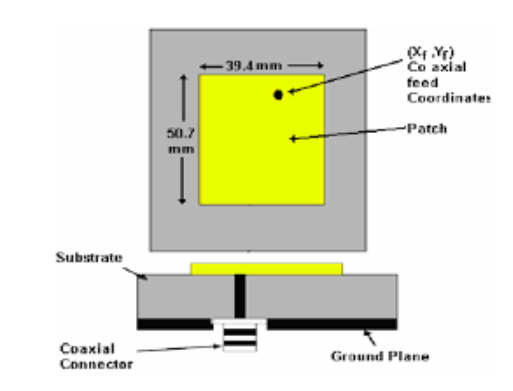
\includegraphics[scale=0.5]{Images/fig1.png}
\caption{پچ مایکرواستریپ با تغذیه ی کواکسیال}
\label{fig1}
\end{figure}
\begin{figure}
	\centering
	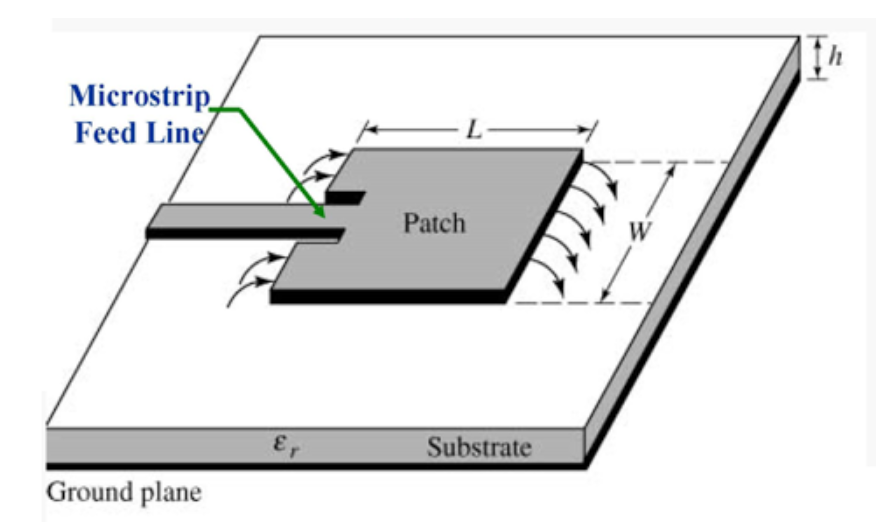
\includegraphics[scale=0.3]{Images/fig2.png}
	\caption{پچ مایکرواستریپ با تغذیه ی خط مایکرواستریپ}
	\label{fig2}
\end{figure}


از میان اشکال مختلف پَچ، انواع مربعی، مستطیلی به دلیل ویژگی‌های تشعشعی مطلوب بیشترین کاربرد را دارند.

\section{معایب آنتن مایکرواستریپ}
بازده پایین، توان پایین، قطبی‌شدگی خالص کم، عملکرد تطبیق ضعیف (فاکتور
$Q$
 بالاتر از ۱۰۰)، تأثیر تغذیه کاذب، و پهنای باند فرکانسی باریک (که در حد یک درصد و در نهایت چند درصد است) را می‌توان از معایب آنتن‌های مایکرواستریپ برشمارد.

البته راهکارهایی مانند افزایش ضخامت زیرلایه، می‌تواند بازده را تا ۹۰ درصد و پهنای باند را تا ۳۵ درصد افزایش دهد. البته با افزایش ضخامت زیرلایه، امواج سطحی
\LTRfootnote{Surface Wave}
 که مطلوب نیستند را نیز باید در نظر گرفت. امواج سطحی به علت تضعیف توان ارسالی مطلوب نیستند. امواج سطحی در زیرلایه انتقال می‌یابند و در ناپیوستگی‌ها و خمیدگی‌ها، مانند نقاط اتصال با صفحه زمین 
\LTRfootnote{Ground Plane}
 ظاهر خواهند شد که مشخصات آنتن (مانند الگوی تشعشع) را تغییر می‌دهد. امواج سطحی وقتی آنتن در یک حفره قرار می‌گیرد قابل صرف‌نظر است.


آنتن مایکرواستریپ خارج از ناحیه عملکرد، اثر الکترومغناطیسی زیادی در فرکانس‌های مشخص خواهد داشت. در سیستم‌های آرایه‌ای حتی در
\lr{VHF}\LTRfootnote{Very High Frequency}
 و
\lr{UHF}\LTRfootnote{Ultra High Frequency}
 بین پهنای باند و نرخ تطبیق، داد و ستد
\LTRfootnote{Trade-off}
  وجود دارد.


\section{انواع تغذیه}
\begin{figure}
	\centering
	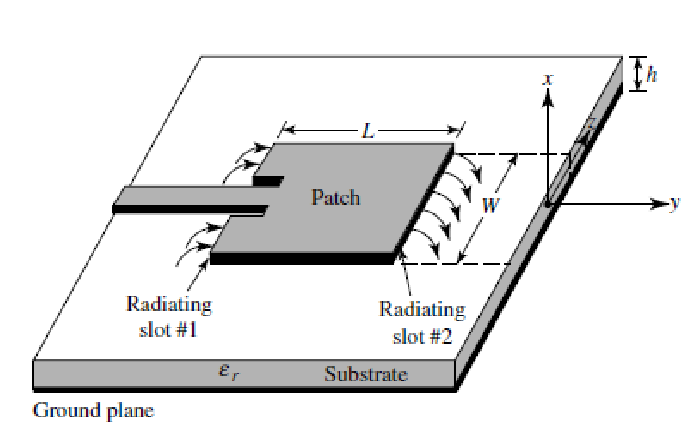
\includegraphics[scale=0.3]{Images/fig3.png}
	\caption{آنتن با تغذیه ی مایکرواستریپ}
	\label{fig3}
\end{figure}
روش‌های متعددی برای تغذیه آنتن‌های مایکرواستریپ وجود دارد که از جمله متداول‌ترین آن‌ها می‌توان به تغذیه توسط خط مایکرواستریپ
\LTRfootnote{Microstrip Line Feed}،
تغذیه کوپلینگ روزنه‌ای
\LTRfootnote{Aperture Coupling}،
 (شکل
\ref{fig4}
)
تغذیه کوپلینگ مجاورتی
\LTRfootnote{Proximity Coupling}
(شکل
\ref{fig5}
)
و تغذیه پروب کواکسیال
\LTRfootnote{Coaxial Probe Feed} 
 (شکل
\ref{fig6}
)
اشاره نمود.  



\subsection{آنتن با تغذیه ی کوپلینگ روزنه ای}
\begin{figure}
	\centering
	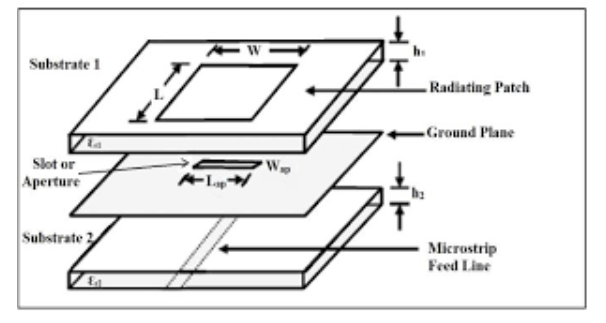
\includegraphics[scale=0.4]{Images/fig4.png}
	\caption{آنتن با تغذیه ی کوپلینگ روزنه ای}
	\label{fig4}
\end{figure}

\subsection{آنتن با تغذیه ی کوپلینگ مجاورتی}
\begin{figure}
	\centering
	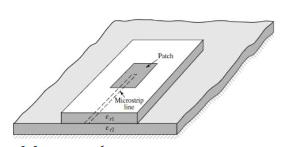
\includegraphics[scale=0.7]{Images/fig5.png}
	\caption{آنتن با تغذیه ی کوپلینگ مجاورتی}
	\label{fig5}
\end{figure}

\subsection{آنتن با تغذیه ی کواکسیال}
در تغذیه آنتن‌های مایکرواستریپ از طریق کابل کواکسیال، هادی مرکزی کابل به پچ و شیلد خارجی کابل به صفحه زمین متصل می‌شود. این روش تغذیه به دلیل سادگی ساخت و امکان تطبیق آسان امپدانس، به طور گسترده‌ای مورد استفاده قرار می‌گیرد. با این حال، این نوع اتصال دارای پهنای باند محدود است و مدل‌سازی دقیق آن در شبیه‌سازی‌ها دشوار می‌باشد.(شکل
\ref{fig6})
\begin{figure}
	\centering
	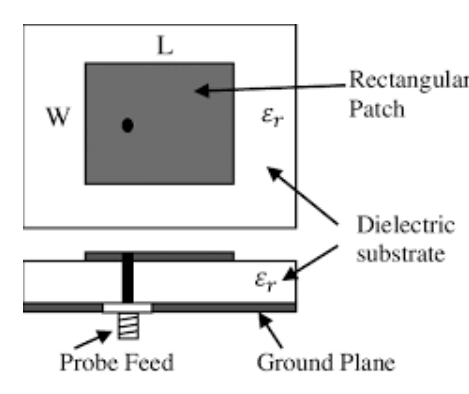
\includegraphics[scale=0.3]{Images/fig6.png}
	\caption{آنتن با تغذیه ی کواکسیال}
	\label{fig6}
\end{figure}


\subsection{آنتن با پچ مستطیلی}
آنتن‌های با پچ مستطیلی به دلیل طراحی ساده، اندازه فشرده و عملکرد پایدار، به‌طور گسترده در سیستم‌های مخابراتی، ماهواره‌ای و راداری مورد استفاده قرار می‌گیرند. در این پژوهش، از روش تغذیه کواکسیال بهره گرفته شده است که در آن هادی مرکزی کابل مستقیماً به پچ و شیلد خارجی به صفحه زمین متصل می‌شود. این روش به دلیل سادگی ساخت، اتلاف پایین و قابلیت تطبیق امپدانس کارآمد، انتخاب شده است؛ هرچند که دارای محدودیت ذاتی در پهنای باند است.(شکل 
\ref{fig7})
\begin{figure}
	\centering
	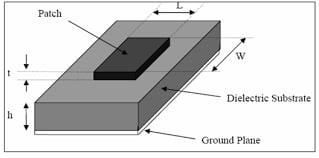
\includegraphics[scale=0.9]{Images/fig7.jpg}
	\caption{آنتن با پچ مستطیلی}
	\label{fig7}
\end{figure}

در این پروژه، از روش تغذیه پروب کواکسیال استفاده شده است که دلیل انتخاب آن، سادگی ساخت، اتلاف کم و قابلیت اطمینان بالا در کاربردهای عملی است. در ادامه، به بررسی دقیق‌تر اصول کاری و ملاحظات طراحی این روش پرداخته خواهد شد.


\section{اثر لبه}

به دلیل محدودیت ابعاد پچ در راستای طول و عرض، میدان‌های الکترومغناطیسی از لبه‌های پچ به بیرون انتشار می‌یابند که این پدیده تحت عنوان اثر لبه‌ای
\LTRfootnote{Fringing Effect}
شناخته می‌شود
\cite{chahar}.
همانطور که در شکل 
\ref{fig8}
نشان داده شده است
\cite{do}،
این اثر منجر به گسترش میدان‌ها در خارج از مرزهای فیزیکی پچ می‌گردد.

\begin{figure}
	\centering
	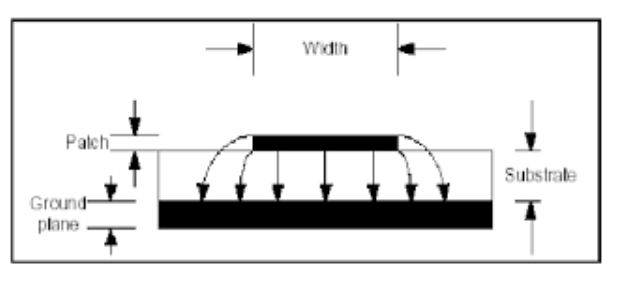
\includegraphics[scale=0.3]{Images/fig8.png}
	\caption{اثر لبه در پچ مایکرواستریپ}
	\label{fig8}
\end{figure}

میزان تراوش میدان از لبه‌ها تابعی از ابعاد هندسی پچ (طول
$L$
 و عرض
$W$)
 و همچنین ویژگی‌های زیرلایه از جمله ارتفاع (
$h$)
 و ثابت دی‌الکتریک (
 $\varepsilon_r$)
 است. برای صفحه اصلی
 $E$،
  این اثر به طور خاص به نسبت
$L$
  و
$\varepsilon_r$
 وابسته می‌باشد.


همانطور که در شکل بالا مشاهده می‌شود، بخش عمده‌ای از خطوط میدان در داخل زیرلایه متمرکز شده‌اند، در حالی که بخشی از آن‌ها به محیط اطراف (هوا) نفوذ می‌کنند. در شرایطی که
$ \frac{W}{h} \gg 1$
 باشد، تراکم خطوط میدان عمدتاً درون زیرلایه رخ می‌دهد. اثر لبه‌ای سبب می‌شود که طول الکتریکی پچ بزرگ‌تر از ابعاد فیزیکی آن به نظر رسد. از آنجایی که بخشی از میدان در هوا و بخشی دیگر در زیرلایه انتشار می‌یابد، یک ثابت دی‌الکتریک مؤثر(
$\varepsilon_{e}$)
 تعریف می‌شود تا تأثیر هر دو محیط به صورت همزمان در محاسبات در نظر گرفته شود. این کمیت به صورت تحلیلی و بر اساس پارامترهای ساختاری آنتن محاسبه شده و نقش اساسی در تعیین دقیق فرکانس تشدید و سایر پارامترهای الکتریکی آنتن ایفا می‌کند.


برای تعریف ثابت دی‌الکتریک موثر، فرض می‌کنیم لایه رسانا با ابعاد اصلی خود (مطابق شکل فوق) در میان زیرلایه قرار گرفته است. ثابت دی‌الکتریکی‌ای که در این حالت، همان مشخصه انتشار حالت قبل را از خود نشان دهد را ثابت دی‌الکتریک موثر(
$\varepsilon_{e}$)
می‌نامند.


اگر ثابت دی‌الکتریک زیرلایه(
$\varepsilon_r$)
بسیار بزرگ باشد، ثابت موثر(
$\varepsilon_{e}$)
به ثابت زیرلایه(
$\varepsilon_{r}$)
نزدیک‌تر است. به علاوه، ثابت موثر تابعی از فرکانس نیز می‌باشد. شکل 
\ref{fig9}
 رابطه بین ثابت موثر دی‌الکتریک و فرکانس را برای سه زیرلایه متفاوت نشان می‌دهد.

\begin{figure}
	\centering
	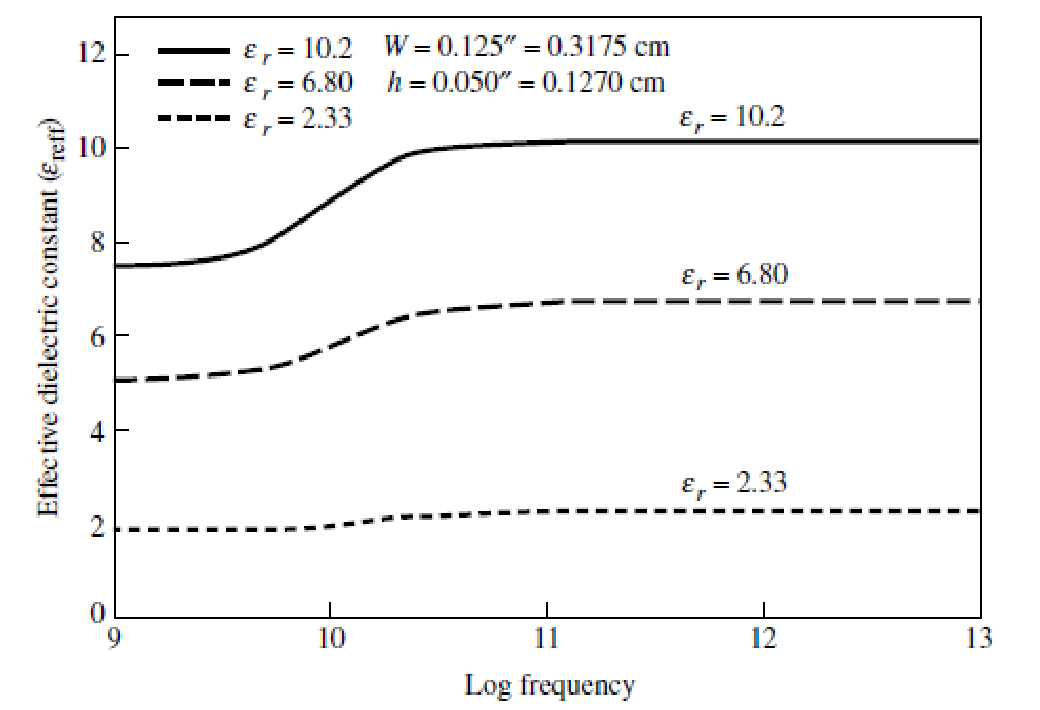
\includegraphics[scale=0.3]{Images/fig9.png}
	\caption{رابطه ی بین ثابت موثر دی الکتریک و فرکانس}
	\label{fig9}
\end{figure}

ثابت موثر دی الکتریک از معادلات 
\ref{eq:eq2}
و
\ref{eq:eq3}
بدست می آید:

\begin{align}
 	\label{eq:eq2}
    \frac{W}{H} < 1	\qquad  \varepsilon_e = \frac{\varepsilon_r+1}{2} + \frac{\varepsilon_r-1}{2} \left[ \left(1+12\frac{H}{W}\right)^{-1/2} + 0.04 \left(1-\frac{W}{H}\right)^2 \right]
\end{align}


\begin{align}
	\label{eq:eq3}
    \frac{W}{H} \geq 1 \qquad \varepsilon_e = \frac{\varepsilon_r+1}{2} + \frac{\varepsilon_r-1}{2} \left(1+12\frac{H}{W}\right)^{-1/2} 
\end{align}


\section{طول موثر، فرکانس تشدید و پهنای باند موثر}
به دلیل اثر حاشیه‌ای
\LTRfootnote{Fringing Effect}،
 طول الکتریکی پَچ به اندازه
$ \delta L$
 افزایش می‌یابد. این افزایش تابعی از ثابت دی‌الکتریک مؤثر(
 $\varepsilon_{e}$)
 و نسبت عرض به ارتفاع
 $W/h$
  زیرلایه است که از رابطه تجربی 
\eqref{eq:eq4}
   محاسبه می‌شود.
\begin{align}
	\label{eq:eq4}
	\frac{\Delta L}{h} = 0.412 \frac{(\varepsilon_{e}+0.3)\left(\frac{W}{h}+0.264\right)}{(\varepsilon_{e}-0.258)\left(\frac{W}{h}+0.8\right)}
\end{align}


\begin{figure}
	\centering
	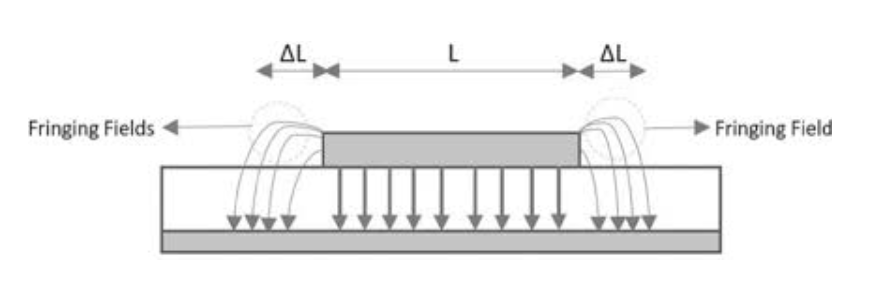
\includegraphics[scale=0.3]{Images/fig10.png}
	\caption{رابطه ی بین ثابت موثر دی الکتریک و فرکانس}
	\label{fig10}
\end{figure}

\begin{figure}
	\centering
	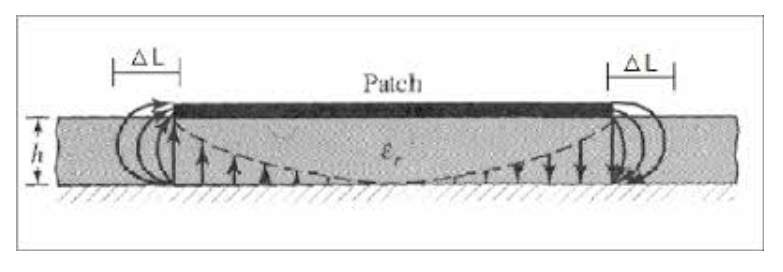
\includegraphics[scale=0.3]{Images/fig11.png}
	\caption{طول های فیزیکی و موثر پچ مایکرواستریپ مستطیلی}
	\label{fig11}
\end{figure}

با در نظر گیری این اثر، طول مؤثر پَچ(
$L_{e}$)
برای محاسبه فرکانس تشدید به صورت 
\eqref{eq:eq5}
 تعریف می‌شود.که در آن 
 $L$
  طول فیزیکی پَچ است.
\begin{align}
	\label{eq:eq5}
	L_{e} = L + 2\delta L
\end{align}

برای مد غالب
$TM_{010}$
فرکانس تشدید به صورت 
\eqref{eq:eq6}
است.
\begin{align}
	\label{eq:eq6}
	(f_r)_{010} = \frac{1}{2L\sqrt{\varepsilon_r}\sqrt{\mu_0\varepsilon_0}} = \frac{v_0}{2L\sqrt{\varepsilon_r}}
\end{align}
$v_0$
سرعت نور در فضای آزاد است.

با در نظرگیری اثر حاشیه‌ای، محاسبه فرکانس تشدید نیازمند اصلاح طول پچ و استفاده از ثابت دی‌الکتریک مؤثر است. فرکانس تشدید برای حالت پایه
$TM_{10}$
 به صورت
\eqref{eq:eq7}
  محاسبه می‌شود.
\begin{align}
	\label{eq:eq7}
	(f_r)_{010} = \frac{1}{2L_{e}\sqrt{\varepsilon_{e}}\sqrt{\mu_0\varepsilon_0}} = \frac{c}{2(L+2\Delta L)\sqrt{\varepsilon_{e}}}
\end{align}

ضریب تراوش
$q$
 به عنوان نسبت فرکانس تشدید واقعی به فرکانس تشدید بدون در نظرگیری اثر حاشیه‌ای به صورت
\eqref{eq:eq8}
  تعریف می‌شود.
\begin{align}
	\label{eq:eq7}
	q = \frac{(f_r)_{\text{actual}}}{(f_r)_{\text{without fringing}}}
\end{align}

با افزایش ارتفاع زیرلایه (
$h$)،
 اثر حاشیه‌ای تشدید شده و موجب افزایش
 $\Delta L$
  و در نتیجه کاهش فرکانس تشدید می‌گردد. این پدیده به‌طور مستقیم بر عملکرد آنتن تأثیر گذاشته و طراحی را به سمت استفاده از مدل‌های دقیق‌تر برای پیش‌بینی رفتار آنتن سوق می‌دهد.












\newpage 
\chapter{آنتن آرایه ای ، تزویج ( کوپلینگ ) و راه های کاهش آن}
\label{ch:2}
\section{مقدمه}
پس از آشنایی با اصول طراحی و تحلیل آنتن‌های مایکرواستریپ تکی، در این فصل به بررسی آرایه‌های آنتن و چالش‌های مرتبط با تزویج متقابل
\LTRfootnote{Coupling}
 بین المان‌های آرایه پرداخته می‌شود. هدف اصلی، تبیین مکانیزم‌های تزویج و ارائه راه‌کارهای عملی برای کاهش اثرات نامطلوب آن در عملکرد آرایه است.
 
\section{آرایه ها و شبکه ی تغذیه}
آرایهٔ آنتنی به مجموعه‌ای از چندین المان تشعشعی گفته می‌شود که به صورت منظم یا نامنظم در کنار یکدیگر قرار گرفته و با تغذیهٔ مناسب، الگوی تشعشعی دلخواه ایجاد می‌کنند. آرایه‌ها معمولاً از ترکیب آنتن‌های ساده‌ای مانند پچ، دیپل یا شکاف ساخته می‌شوند و با تنظیم دامنه و فاز جریان تغذیهٔ هر المان، می‌توان شکل پرتو را کنترل و در جهات مختلف هدایت کرد.


آرایه‌ها کاربردپذیری بالایی دارند و برای تولید الگوهای تشعشعی مورد نظر که با یک المان منفرد قابل دستیابی نیستند، استفاده می‌شوند. به علاوه، برای چرخاندن پرتو یک سیستم آنتن، افزایش سمت‌گرایی
\LTRfootnote{Directivity}
 و انجام کارهایی که با المان‌های تکی دشوار است، به‌کار گرفته می‌شوند. به همین دلیل، آرایه‌ها نقش کلیدی در رادارها، سیستم‌های مخابرات ماهواره‌ای،
 \lr{5G}
  و سامانه‌های
  \lr{MIMO}
   ایفا می‌کنند.
   
   
   آرایه ها به دو صورت میتوانند تغذیه شوند:‌ تغذیه ی سری و موازی. البته به صورت ترکیبی هم ممکن است.
   

\begin{figure}[t]
	\centering
	\begin{subfigure}{0.3\textwidth} % width of left subfigure
		
\includegraphics[scale=0.2]{Images/aaa.jpg}
		\caption{تغذیه سری} % subcaption
		\label{fig12}
	\end{subfigure}
	\vspace{1em} % here you can insert horizontal or vertical space
	\begin{subfigure}{0.3\textwidth} % width of right subfigure
		
\includegraphics[scale=0.2]{Images/aaa.jpg}
		\caption{تغذیه موازی} % subcaption
		\label{fig13}
	\end{subfigure}
		\vspace{1em} % here you can insert horizontal or vertical space
	\begin{subfigure}{0.3\textwidth} % width of right subfigure
		
\includegraphics[scale=0.2]{Images/aaa.jpg}
		\caption{تغذیه سری موازی} % subcaption
		\label{fig14}
	\end{subfigure}
	\caption{}
\end{figure}


در این روش که برای تقسیم توان به توان‌های
$ 2^n$
 (یعنی ۲، ۴، ۸، ۱۶ و ...) استفاده می‌شود، تقسیم توان با استفاده از خطوط تغذیه باریک‌شونده
\LTRfootnote{Tapered Lines}
 مطابق شکل زیر انجام می‌شود تا امپدانس المان‌های پَچ (معمولاً ۱۰۰ اهم) را به امپدانس ورودی استاندارد (۵۰ اهم) تطبیق دهد.



\begin{figure}
	\centering
	
\includegraphics[scale=0.3]{Images/aaa.jpg}
	\caption{خطوط باریک شونده}
	\label{fig15}
\end{figure}

به علاوه میتوان با مبدل های امپدانس ربع طول موج هم این کار را انجام داد:
\begin{figure}
	\centering
	
\includegraphics[scale=0.3]{Images/aaa.jpg}
	\caption{مبدل یک چهارم طول موج}
	\label{fig16}
\end{figure}

آرایه‌های تغذیه سری را می‌توان به راحتی با استفاده از مدل چاپی نوری برای المان‌های تشعشعی و شبکه تغذیه ساخت. البته این روش به آرایه با پرتو ثابت یا آرایه‌هایی که با تغییر فرکانس اسکن می‌شوند محدود می‌شود، ولی می‌توان از این تکنیک برای آرایه‌های خطی صفحه‌ای با پلاریزاسیون تکی یا دوگانه استفاده کرد. همچنین هرگونه تغییر در یکی از المان‌ها یا خطوط تغذیه، عملکرد بقیه را تحت تأثیر قرار می‌دهد. بنابراین در یک طراحی، در نظر گرفتن این اثرات و سایر اثرات مانند تلفیق متقابل و بازتابش‌های داخلی مهم است.


آرایه‌های تغذیه مشارکتی، متداول و دارای کاربردهای متنوعی هستند. با این روش، طراح کنترل بیشتری روی تغذیه هر المان (دامنه و فاز) دارد و این روش برای آرایه‌های فاز اسکن‌کننده، آرایه‌های چندپرتوئی یا آرایه‌های با پرتو شکل‌داده‌شده، ایده‌آل است. فاز هر المان را با استفاده از شیفت‌دهنده‌ها می‌توان کنترل کرد و دامنه را با استفاده از تقویت‌کننده‌ها و تضعیف‌کننده‌ها می‌توان تحت کنترل قرار داد.


نکته قابل توجه این است که چه در تغذیه سری و چه در مشارکتی، تشعشع از خط تغذیه قابل ملاحظه و مهم است که پلاریزاسیون را متقاطع و سطح لوب کناری آرایه را افزایش می‌دهد. که هر دو را می‌توان با جداسازی شبکه تغذیه از صفحه تشعشع‌کننده آرایه بهبود بخشید که این کار را می‌توان با استفاده از تغذیه‌های پروبی یا تغذیه روزنه‌ای انجام داد.


\section{تزویج}
یکی از مسائل مهم در طراحی آرایه‌های آنتنی، تزویج متقابل میان عناصر آرایه است. هنگامی که المان‌ها در فاصله‌ای کمتر از چندین طول‌موج قرار گیرند، میدان‌های الکترومغناطیسی هر المان بر سایر المان‌ها اثر می‌گذارد. این پدیده باعث می‌شود که جریان‌های القاشده روی المان‌های مجاور تغییر کنند و در نتیجه امپدانس ورودی، بهره و الگوی تابش کل آرایه دچار تغییر شود.


این تزویج باعث بوجود آمدن تغییرات زیر میشود : 

\begin{itemize}
	\item{
	انحراف امپدانس ورودی از مقدار طراحی شده
	} 
	\item{
	کاهش بهره و بازدهی آرایه
	}
	\item{
	تغییر در الگوی تشعشعی (افزایش
	\lr{sidelobe}
	ها).
	}
	\item{
	محدودیت پهنای باند عملیاتی.
	}
\end{itemize}

دو نوع چیدمان برای پَچ‌های میکرواستریپ وجود دارد: یکی در راستای محور
$ y$
 و دیگری در راستای محور
 $ x$
 (شکل
 \ref{fig17}).

هدف از میدانی که با تنظیم خطوط تغذیه در طول
$ y$
 قرار داده می‌شوند، این است که میدان‌های الکتریکی تشعشعی در تشدید در طول
 $ L$،
  پلاریزاسیون خطی ایجاد کند. 


این بدین معنی است که میدان‌های الکتریکی تشعشع‌یافته در طول
$ y$
 بیشتر پلاریزه می‌شوند و این نیز به معنای تزویج بیشتر در این وضعیت است. در نتیجه، این وضعیت نشان می‌دهد که چیدمان پَچ در طول محور
 $ x$،
  تزویج متقابل
\LTRfootnote{Mutual Coupling}
 را کاهش می‌دهد.
 
\begin{figure}
	\centering
	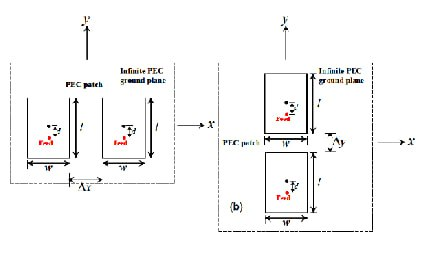
\includegraphics[scale=1]{Images/fig17.jpg}
	\caption{قرار گیری پچ ها در راستای 
		$x$ 
		و 
		$y$}
	\label{fig17}
\end{figure}

میتوان نشان داد که تزویج بین دو پچ تابع مکان یکی نسبت به دیگریست. برای این امر به مقاله ی
\cite{carver1981microstrip}
 استناد میکنیم. در این مقاله ثابت شده که با افزایش فاصله بین دو پچ ، تزویج متقابل نیز کاهش میابد. 

\begin{figure}
	\centering
	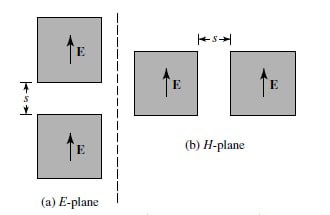
\includegraphics[scale=1]{Images/fig18.jpg}
	\caption{آرایش صفحه های E و H آنتن های مایکرواستریپ}
	\label{fig18}
\end{figure}

در نمودار 
\ref{fig19}
 تغییرات تزویج متقابل بین دو پچ در فواصل مختلف در دو آرایش E و H از مقاله ی 
 \cite{carver1981microstrip}
  نمایش داده میشود. 

\begin{figure}
	\centering
	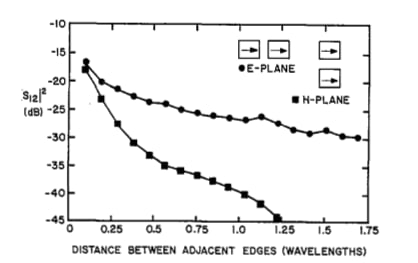
\includegraphics[scale=1]{Images/fig19.jpg}
	\caption{نمودار تزویج متقابل بین دو پچ در آرایش E و H}
	\label{fig19}
\end{figure}

در شکل فوق ابعاد آنتن به صورت زیر میباشد:
\begin{align}
	\label{eq:eq8}
	W = 10.57 \text{cm}, L = 6.55 \text{cm}, h = 0.1588 \text{cm}, \varepsilon_r = 2.55, f_r = 1.410 \text{MHz}
\end{align}

ابعاد
$ L$
 و
 $ W$
  از فرمول های 
  \ref{eq:eq9}
   تبعیت میکنند:
\begin{align}
	\label{eq:eq9}
	W = \frac{c}{2f_r\sqrt{\frac{\varepsilon_r+1}{2}}}
\end{align}
که در آن:
\begin{itemize}
	\item{$W$:
	عرض پچ(بر حسب متر)
	}
	\item{$c$:
	سرعت نور در خلاء
	}
	\item{$f_r$:
	فرکانس رزونانس (بر حسب هرتز)
	}
	\item{$\varepsilon_{r}$:
	ثابت دی الکتریک نسبی زیرلایه
	}
\end{itemize}


\begin{align}
	\label{eq:eq10}
	\varepsilon_{\text{eff}} = \frac{\varepsilon_R+1}{2} + \frac{\varepsilon_R-1}{2}\left[\frac{1}{\sqrt{1+12\left(\frac{h}{W}\right)}}\right]
\end{align}

\begin{align}
	\label{eq:eq11}
	\text{Length} = \frac{c}{2f_0\sqrt{\varepsilon_{e}}} - \left(2 \times \left[0.412h\frac{(\varepsilon_{e}+0.3)\left(\frac{W}{h}+0.264\right)}{(\varepsilon_{e}-0.258)\left(\frac{W}{h}+0.8\right)}\right]\right)
\end{align}

که با جایگذاری به تقریبا به همین اعداد میرسیم.


در تزویج بین دو پَچ مستطیلی، اگر المان‌ها هم‌راستا در صفحه E باشند، این آرایش، آرایش صفحه E نامیده می‌شود و اگر هم‌راستا در صفحه H باشند، این آرایش، آرایش صفحه H نام خواهد گرفت.

در آرایش صفحه E، معمولاً برای فواصل بسیار کوچک(
$s < 0.10\lambda$)،
 بیشترین تزویج را نشان می‌دهد، در حالی که در آرایش صفحه H، معمولاً برای فواصل بزرگ(
 $s > 0.10\lambda$)،
  کمترین تزویج را نشان می‌دهد. فاصله‌ای که در آن تزویج یک صفحه از دیگری پیشی می‌گیرد، به خواص الکتریکی و ابعاد هندسی آنتن مایکرواستریپ بستگی دارد.

به طور کلی، تزویج متقابل بیشتر به میدان‌هایی که در امتداد فصل‌مشترک هوا با دی‌الکتریک وجود دارند مربوط میشود. این میدان ها میتوانند به امواج فضایی(با تغییرات شعاع
$1/\rho$)
امواج مرتبه بالاتر(با تغییرات شعاع
$1/\rho^2$)
امواج سطحی(با تغییرات شعاع
$1/\rho^{\frac{1}{2}}$)
وامواج نشطی(با تغییرات شعاع
$\exp{-\lambda_{p}/\rho^{\dfrac{1}{2}}}$)
تجزیه شوند. به دلیل تغییرات شعاعی کروی، امواج فضایی و مرتبه بالاتر برای فواصل کوچک و امواج سطحی برای فواصل بزرگ غالب می‌شوند.


امواج سطحی که داخل دی‌الکتریک وجود دارد، در آن منتشر می‌شود و تحریک آن‌ها تابعی از ضخامت دی‌الکتریک است. برای یک پَچ مستطیلی، میدان‌ها در جهت انتشار در امتداد صفحه E از نوع TM و در امتداد صفحه H از نوع TE هستند. در آرایش صفحه E، همانطور که در شکل فوق نشان داده شده، المان‌ها در راستای صفحه E قرار دارند و در فاصله بین المان‌ها میدان از نوع TM است. یک تحریک موج سطحی قوی‌تر بین المان‌ها وجود دارد و تزویج بزرگتر است. اما در صفحه H این گونه نیست و تحریک موج سطحی قوی وجود ندارد و تزویج کمی وجود دارد. با افزایش ضخامت زیرلایه که باعث تحریک موج سطحی TE مرتبه بالاتر می‌شود، این تزویج تغییر می‌کند.






























\newpage 
\chapter{ ساختار زمین ناقص و فراماده و تاثیر آنها بر کاهش تزویج}
\label{ch:3}
\section{مقدمه}
در این فصل با پیاده سازی ساختار ارائه شده در مقاله
\cite{carver1981microstrip}
و یک طرح فراماده مشهور تلاش بر کاهش کوپلینگ شده که در ادامه با توضیح هر کدام ساختار را برسی میکنیم.

\section{ساختار زمین ناقص}
ساختار زمین ناقص  با ایجاد نقص‌های مهندسی‌شده در صفحه زمین، توزیع جریان‌های سطحی را تغییر داده و باعث ایجاد خواص ممنوعه باندی
\LTRfootnote{Band-Stop}
 در پاسخ فرکانسی می‌شود. این ویژگی به‌طور مستقیم بر کاهش تزویج متقابل از طریق مهار انتشار امواج سطحی تأثیر می‌گذارد.
 
 
 ساختار DGS را می‌توان با یک مدار LC موازی مدلسازی کرد که در فرکانس رزونانس، امپدانس بالایی را ایجاد می‌کند و باعث مسدودسازی سیگنال می‌شود. مقادیر سلف ($L$) و خازن ($C$) به هندسه و ابعاد نقص ایجاد شده در صفحه زمین بستگی دارد.
 رابطه فرکانس رزونانس:
 \begin{align}
 	\label{eq:eq12}
	f_r = \frac{1}{2\pi\sqrt{LC}}
 \end{align}
 
 این مدل مدار معادل، درک بهتری از رفتار فرکانسی ساختار DGS و تأثیر آن بر کاهش کوپلینگ ارائه می‌دهد.
 
 
 \begin{figure}
 	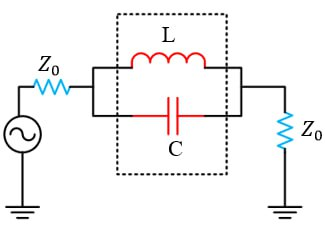
\includegraphics[scale=0.5]{Images/fig26.jpg}
 	\caption{معادل مداری ساختار زمین ناقص}
 	\label{fig26}
 \end{figure}
 
 در مقاله ی مد نظر ساختار انتخابی به صورت زیر میباشد: 
 
\begin{figure}
	\centering
	\begin{subfigure}{0.5\textwidth} % width of left subfigure
		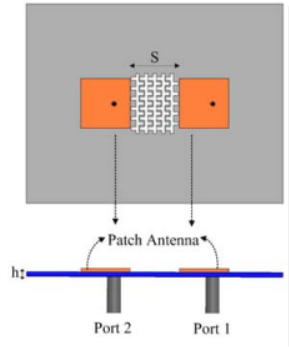
\includegraphics[scale=0.25]{Images/fig27.png}
		\caption{نمای بالایی و کناری از دو پچ آنتن به همراه DGS در صفحه ی زمین} % subcaption
		\label{fig27}
	\end{subfigure}
	\vspace{1em} % here you can insert horizontal or vertical space
	\begin{subfigure}{0.5\textwidth} % width of right subfigure
		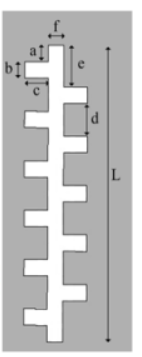
\includegraphics[scale=0.25]{Images/fig28.png}
		\caption{ارامتر های یک سلول DGS} % subcaption
		\label{fig28}
	\end{subfigure}
	\caption{}
\end{figure}
 
 
 با توجه به اینکه طراحی ارائه شده در مقاله مرجع
 \cite{carver1981microstrip}
 برای فرکانس کاری ۵ گیگاهرتز بهینه‌سازی شده است، جهت استفاده از این ساختار در فرکانس کاری مورد نظر این پروژه (۱.۴ گیگاهرتز)، لازم است ابعاد هندسی ساختار DGS به صورت متناسب اسکیل شوند. از آنجایی که ابعاد ساختارهای الکترومغناطیسی با طول موج رابطه مستقیم دارند، ضریب مقیاس ($\alpha$) از نسبت فرکانس‌ها محاسبه می‌شود: 
 
  \begin{align}
 	\label{eq:eq13}
 	\alpha = \frac{f_{\text{ref}}}{f_{\text{new}}} = \frac{5}{1.4} \approx 3.571
 \end{align}
 
 که در آن ۵ گیگ فرکانس کاری مقاله و 1.4 فرکانس جدید میباشد و در نتیجه ابعاد سلول DGS مقاله باید در 3.57 ضرب شوند.
 ابعاد قبل و بعد از محاسبه به صورت زیر میباشند : 
 
 

%دستوراتی برای به حالت عادی در آمدن اندازه فونت‌ها و فاصله بین خطوط
\normalsize
%ایجاد «مراجع»
\bibliographystyle{ieeetr-fa}
\bibliography{MHBReference}

\newpage
\thispagestyle{empty}
\begin{latin}
\textbf{Abstract:}
Microstrip antennas are widely used in communication systems due to their simple fabrication and small size. However, their use in arrays leads to mutual coupling between elements, which results in consequences like gain reduction and distortion of the radiation pattern. In this study, to investigate and reduce this effect, after introducing microstrip and array antennas, we first reproduced the classical model, which included two rectangular patches at different distances. Then, based on the Carver article, at a distance of a quarter wavelength at a frequency of 1.41 GHz, a DGS (Defected Ground Structure) was designed and applied to improve mutual coupling. Furthermore, a metasurface was placed between the two antennas at a distance from the antenna's plane to create a stopband for surface waves, further reducing mutual coupling. Simulation results in HFSS showed that the combination of the DGS and metasurface led to a reduction of about 32 dB in
$\vert\bm{S}_{21}\vert$
, while 
$\vert\bm{S}_{11}\vert$
and the primary radiation pattern remained almost constant. These results demonstrate the effectiveness of meta-structures in improving the performance of microstrip arrays.



\textbf{keywords}: 
Microstrip antenna, Mutual coupling, Coupling reduction, Patch antennas, Micropatch antennas
\end{latin}
\newpage
\newpage
\thispagestyle{empty}
\vspace*{-28mm}

\centerline{
\includegraphics[scale=0.5]{./Images/general/logo_en.png}}
\begin{latin}
\begin{center}
\large
\vspace{-1mm}
\textbf{School of Engineering}
\\[3cm]
\textbf{Mutual coupling reduction between two microstrip patch antenna}
\\[1.5cm]
Undergraduate Final Project Report
\\[4cm]
By: 
\\[0.5cm]
Mohammad Hassan Beheshti
\\[1cm]
Supervisor:
\\[0.5cm]
Dr. Hamid Reza Hassani
\\[2cm]
September 2025

\end{center}
\end{latin}
\end{document} 
